\documentclass[a4paper,12pt]{article}
\usepackage[margin=25mm]{geometry}
\usepackage{amsmath}
\usepackage{amsfonts}
\usepackage{amssymb}
\usepackage{setspace}
\usepackage{fancyhdr,natbib}



\usepackage{textgreek}
\usepackage{graphicx}
\pagenumbering{gobble}
\usepackage[T1]{fontenc}
\usepackage[utf8]{inputenc}
\usepackage{libertine}
\usepackage{libertinust1math}
\usepackage{verbatim}
\usepackage{gb4e}

\title{Testing Tolerance Principle on Corpus Data}
\author{ }
\date{}
\begin{document}
\maketitle

\section{Introduction}
 Moreover, some pronouns, such as \textit{me/I} and \textit{her/she}, are more vulnerable to case errors than other pronouns \citep[e.g.][]{schutze1996subject,rispoli1998,rispoli1999,pine2005testing}. There is individual variation by child as well. Some children never produce any pronoun case errors; whereas some make errors on one particular pronoun, and some produce all types of errors \citep{rispoli2005}.  

Researchers have provided a wide range of explanations for pronoun case errors. From a theoretical perspective, pronoun case errors occur when the children fail to check both tense and agreement in their utterances according the to Agreement/Tense Omission Model (\textsc{atom}) \citep{wexler1998very,wexler1998subject}. The \textsc{atom} successfully explains the pattern in which the verb accompanying an incorrect pronoun is usually untensed; however, it fails to account for the fact that different pronouns yielf different numbers of errors. Taking children's production into consideration,  \cite{rispoli1998,rispoli1999,rispoli2005} has proposed a  \textsc{paradigm building} model:for each pronoun, case, person, and number form a 3x3 paradigm. Young children have difficulties accessing all forms of pronouns in the paradigm, and thus make pronoun errors. The \textsc{paradigm building} model explains variability in children's pronoun error production since lexical retrieval of a certain pronoun could fail for various reasons. Many researchers suggest that parents' input should also play a part in pronoun case errors. The distribution patterns of the pronoun, such as \textit{Let \underline{me do} it} and \textit{\underline{Her drink} is over there}, can be misleading and result in children's pronoun case errors \citep[e.g.][]{budwig1996influences,tomasello2000,tomasello2003, ambridge2006testing,kirjavainen2009can}.

\section{Objectives}
This paper will investigate pronoun case errors in children's production by conducting a comprehensive corpus analysis on all the available data of English-speaking children on \textsc{childes} \citep{macwhinney2014childes}. First, this paper will review how often does pronoun case errors occur in children's utterances. Although it is treated as a common error in children's speech, the frequency of pronoun case error varies largely from study to study, depending on how the data were collected (corpus data or experimental data) and how the data were coded. This paper will review the frequency of case errors reported in the previous studies and compare them to the error rate found in all the corpora used in this study in order to determine the nature and number of pronoun case errors.

Second, this paper will examine the \textsc{atom} model, the \textsc{paradigm building} model and the input-driven hypothesis using the same set data. In the previous studies, researchers either collected their own data or used different corpora to test their hypotheses. It is necessary to evaluate different theories on the same set of data in order to control for collection bias or limitations of small sample size. 

Third, this paper will provide a hypothesis about how children acquire pronoun case in the first place. Cases are used to mark different relationship between arguments, which is a more abstract grammatical feature to learn compared to plural forms or tense marking. Yet young children are able to produce the correct form of a pronoun in different argument positions. It would be worthwhile to ask the question: how do children acquire this abstract feature at such a young age? This study is going to test two hypotheses of the acquisition of pronoun case. From a theoretical perspective, the children could derive different cases through argument structure. Nominative case and accusative case could be differentiated at the sentential level, such that the former is associated with the subject and the latter case is associated with the object. In addition, children could also acquire cases through statistical learning. Nominative case, accusative case and genitive case have different distributional patterns in speech, which difference could be utilized by children to acquire different cases. 

\section{Methodology}
\subsection{Corpora}
To avoid the limitation of small sample size and selection bias, this study will conduct a comprehensive corpus analysis of speech from monolingual English-speaking children from roughly ages two to four. That includes 46 children with longitudinal recordings and 211 children with cross-sectional recordings (see Table 1 and Table 2 in Appendix).
\subsection{Data Coding}
This study will apply the \textsc{nltk} python package to automatically extract data from the annotated corpora in \textsc{childes}. \textsc{childes} uses MOR and GRASP programs to annotate part-of-speech taggers and dependency grammatical relations for all transcripts. The MOR program produces the \textit{\%mor} tier, in which part-of-speech tags stand in one-to-one correspondence with the word in the transcript line. The GRASP program produces the \textit{\%gra} tier which represents grammatical relations. For English data, the automated annotation system has been reported to have high-level accuracy: the MOR program reaches 97\% of accuracy and the precision for determining subject and object relation is reportedly 95.8\% and 94.1\% for GRASP output \citep{macwhinney2012morphosyntactic,sagae2010morphosyntactic}.  Below is an excerpt from Eve in Brown corpus that exemplifies the \textit{\%mor} tier and \textit{\%gra} tier.
\begin{exe}
\ex \gll *CHI: when me see he again ?\\
\%mor: conj|when pro:obj|me v|see pro:sub|he adv|again ? \\
\%gra: 1|3|LINK 2|3|SUBJ 3|0|ROOT 4|3|OBJ 5|4|JCT 6|3|PUNCT \\
(Brown/Eve/020100.xml)

\ex \gll *CHI:	my find paper .\\
	\%mor:	det:poss|my v|find n|paper .\\
	\%gra:	1|2|SUBJ 2|0|ROOT 3|2|OBJ 4|2|PUNCT\\
(Brown/Adam/020304.xml)
\end{exe}

A pronoun case error is determined by comparing the taggers on the \textit{\%mor} tier and the \textit{\%gra} tier. For example, in sentence (4), \textit{me} is tagged as \textit{pro:obj} on the \textit{\%mor} tier indicating that it's an accusative cased pronoun. In the  \textit{\%gra} tier, it is tagged as \textit{SUBJ}, indicating it is used as in the subject position. The mismatch between the taggers in \textit{\%mor} tier and \textit{\%gra} tier determines that the target pronoun is an error. 

\section{Implications}

There is a rich literature on children's pronoun case errors, but some issues are unsettled because of methodological limitations. With a comprehensive corpus analysis, this study can settle questions, such as when and how often do pronoun case errors occur in children's speech and how prevalent such errors are. In addition, this study will evaluate how well existing theories handle the same set of corpus. That could provide insights about the pros and cons of usage-based, input-based and generative-linguistics-based hypotheses about acquisition. Besides finding the best explanations for pronoun case errors, this study also attempts to answer how do children acquire pronoun case by comparing linguistically-based hypothesesf and statistical learning approaches. 

\newpage
\appendix
\section*{Appendix}
\newpage
\section*{Appendix}
\begin{figure}[!htb]
\begin{minipage}{0.48\linewidth}
    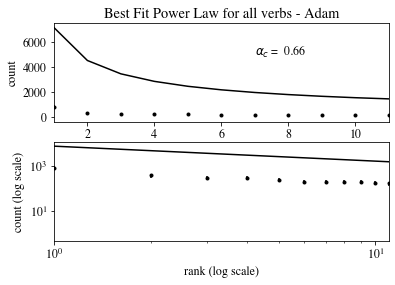
\includegraphics[scale=0.4]{AAC.png}
    \caption{Distribution of Adam's Verbs}
\end{minipage}
\begin{minipage}{0.54\linewidth}
    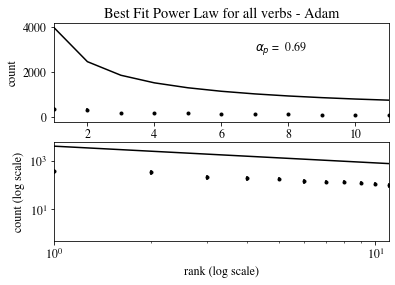
\includegraphics[scale=0.4]{AAP.png}
    \caption{Distribution of Adam's mother's verbs}
\end{minipage}
\end{figure}
\vspace{-2em}
\begin{figure}[!htb]
\begin{minipage}{0.48\linewidth}
\centering
    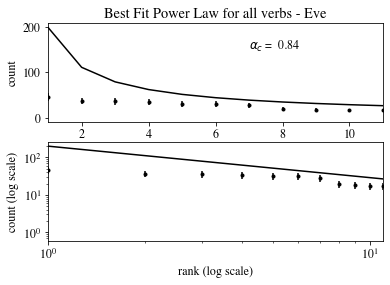
\includegraphics[scale=0.4]{EAC.png}
    \caption{Distribution of Eve's Verbs}
\end{minipage}
\begin{minipage}{0.53\linewidth}
\centering    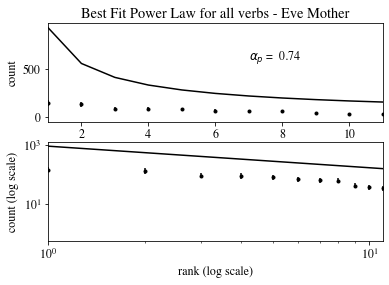
\includegraphics[scale=0.4]{EAP.png}
    \caption{Distribution of Eve's mother's verbs}
\end{minipage}
\end{figure}
\vspace{-2em}
\begin{figure}[!htb]
\begin{minipage}{0.5\linewidth}
    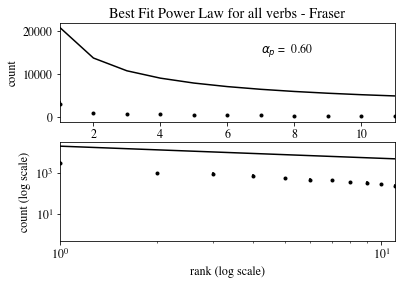
\includegraphics[scale=0.4]{FAC.png}
    \caption{Distribution of Fraser's Verbs}
\end{minipage}
\begin{minipage}{0.55\linewidth}
    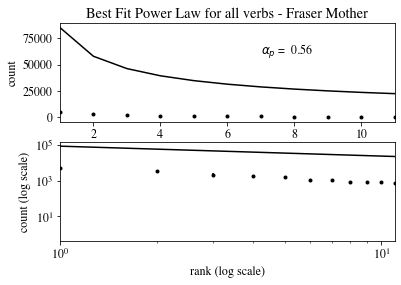
\includegraphics[scale=0.4]{FAP.png}
    \caption{Distribution of Fraser's mother's verbs}
\end{minipage}
\end{figure}
\vspace{-2em}
\begin{figure}[!htb]
\begin{minipage}{0.5\linewidth}
    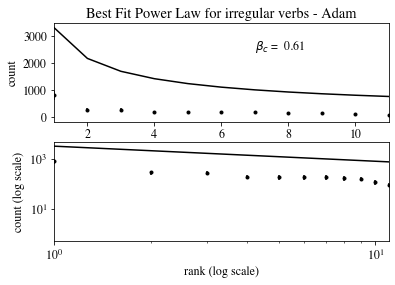
\includegraphics[scale=0.4]{ABC.png}
    \caption{Distribution of Adam's Irregular Verbs}
\end{minipage}
\begin{minipage}{0.5\linewidth}
\centering    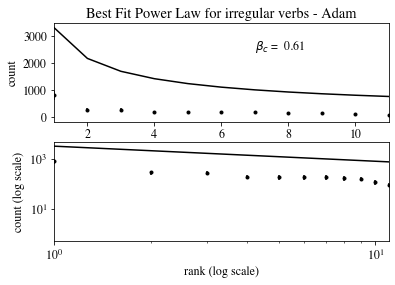
\includegraphics[scale=0.4]{ABC.png}
    \caption{Distribution of Ada's mother's Irregular verbs}
\end{minipage}
\end{figure}
\vspace{-2em}
\begin{figure}[!htb]
\begin{minipage}{0.5\linewidth}
    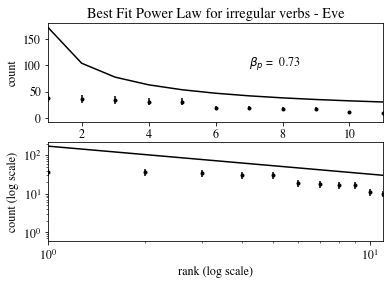
\includegraphics[scale=0.4]{EBC.png}
    \caption{Distribution of Eve's Irregular Verbs}
\end{minipage}
\begin{minipage}{0.5\linewidth}    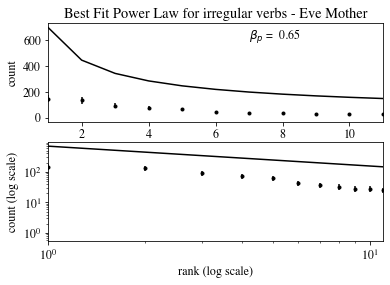
\includegraphics[scale=0.4]{EBP.png}
    \caption{Distribution of Eve's mother's Irregular verbs}
\end{minipage}
\end{figure}
\vspace{-2em}
\begin{figure}[!htp]
\begin{minipage}{0.5\linewidth}
    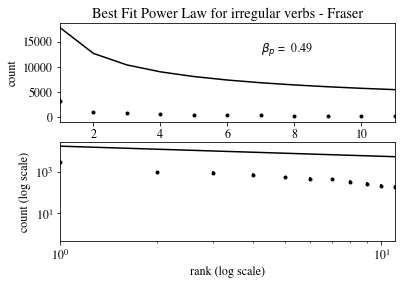
\includegraphics[scale=0.4]{FBC.png}
    \caption{Distribution of Fraser's Irregular Verbs}
\end{minipage}
\begin{minipage}{0.5\linewidth}
    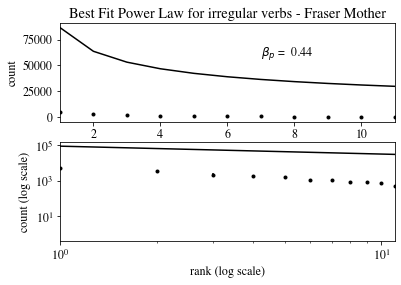
\includegraphics[scale=0.4]{FBP.png}
    \caption{Distribution of Fraser's mother's Irregular verbs}
\end{minipage}
\end{figure}

\newpage
\bibliography{bib}
\bibliographystyle{apalike}
\end{document}
